\textbf{Fruiting in \textsl{Dictyostelium}} In the plate inoculated the \textsl{Dictyostelium}, \textsl{Dictyostelium} slug grew in the direction of the smeared \textsl{E. coli} (Fig.\ref{Fig.sub.1}). In the plate without treatment, there were no other bacteria, except \textsl{E. coli} (Fig.\ref{Fig.sub.2}).

\begin{figure}[H]
    \centering
    \subfigure[]{
    \label{Fig.sub.1}
    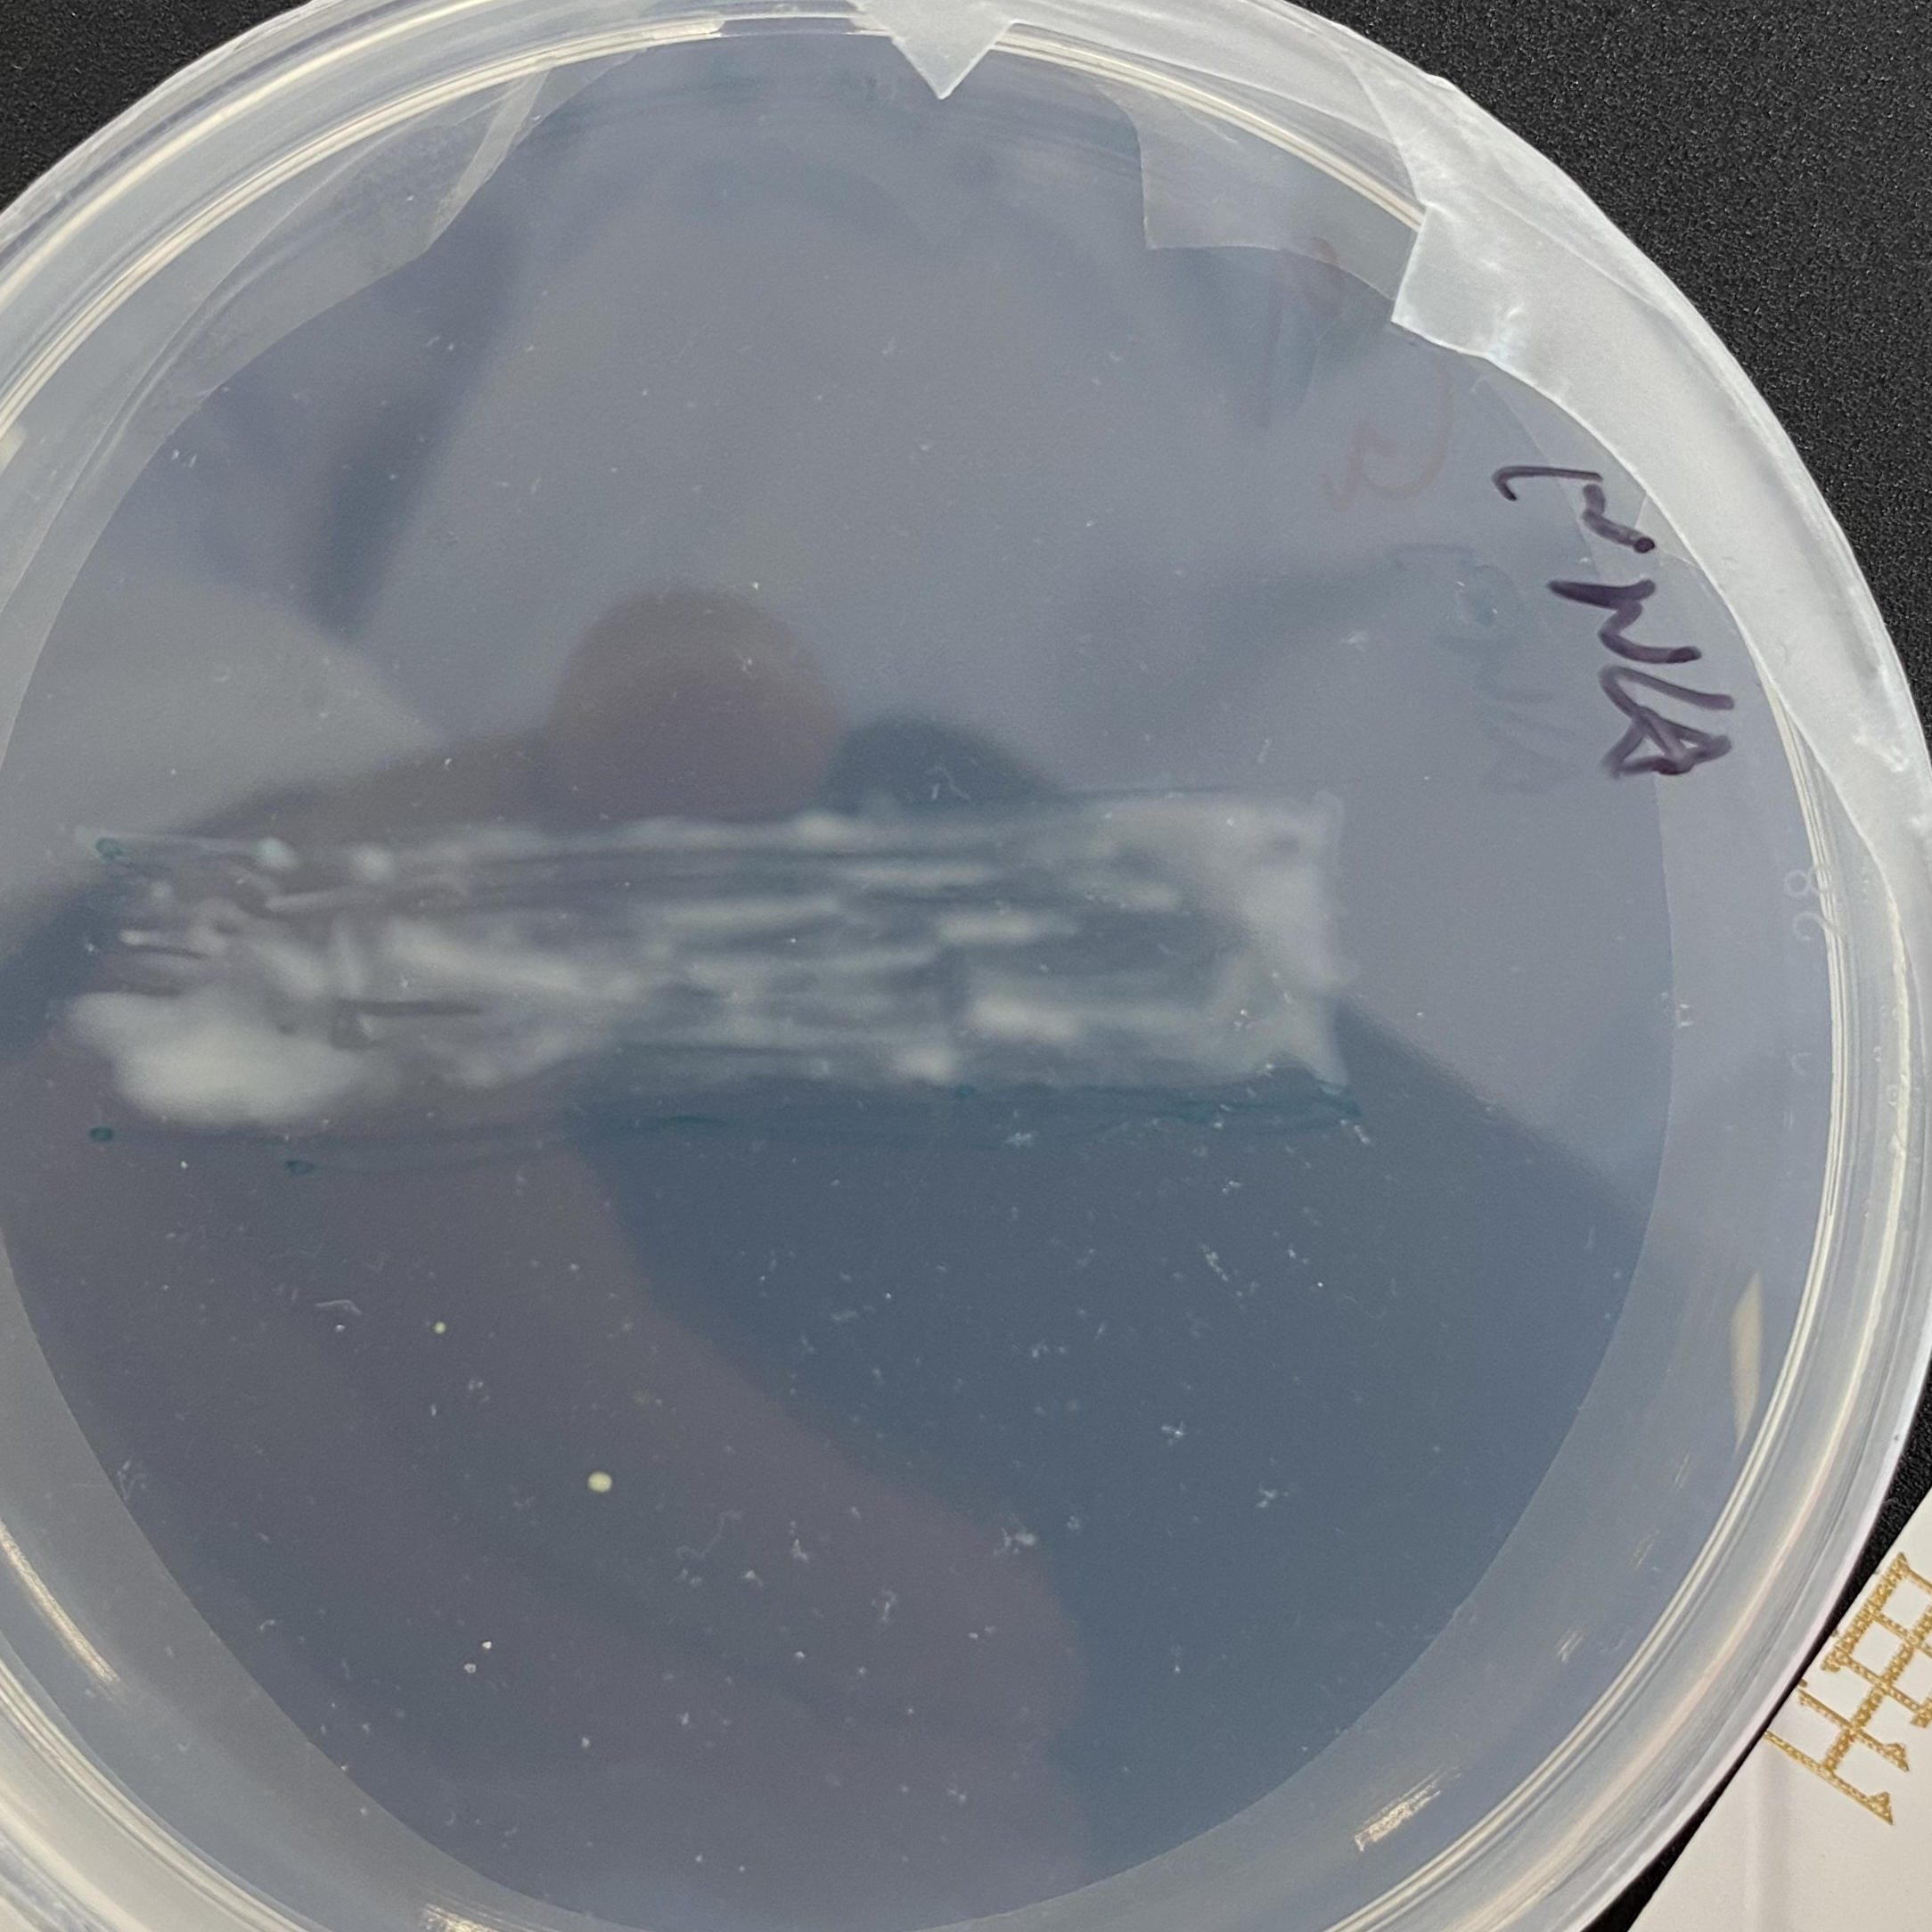
\includegraphics[width=0.26\textwidth, height=0.25\textwidth]{figures/p1E.jpg}}
    \subfigure[]{
    \label{Fig.sub.2}
    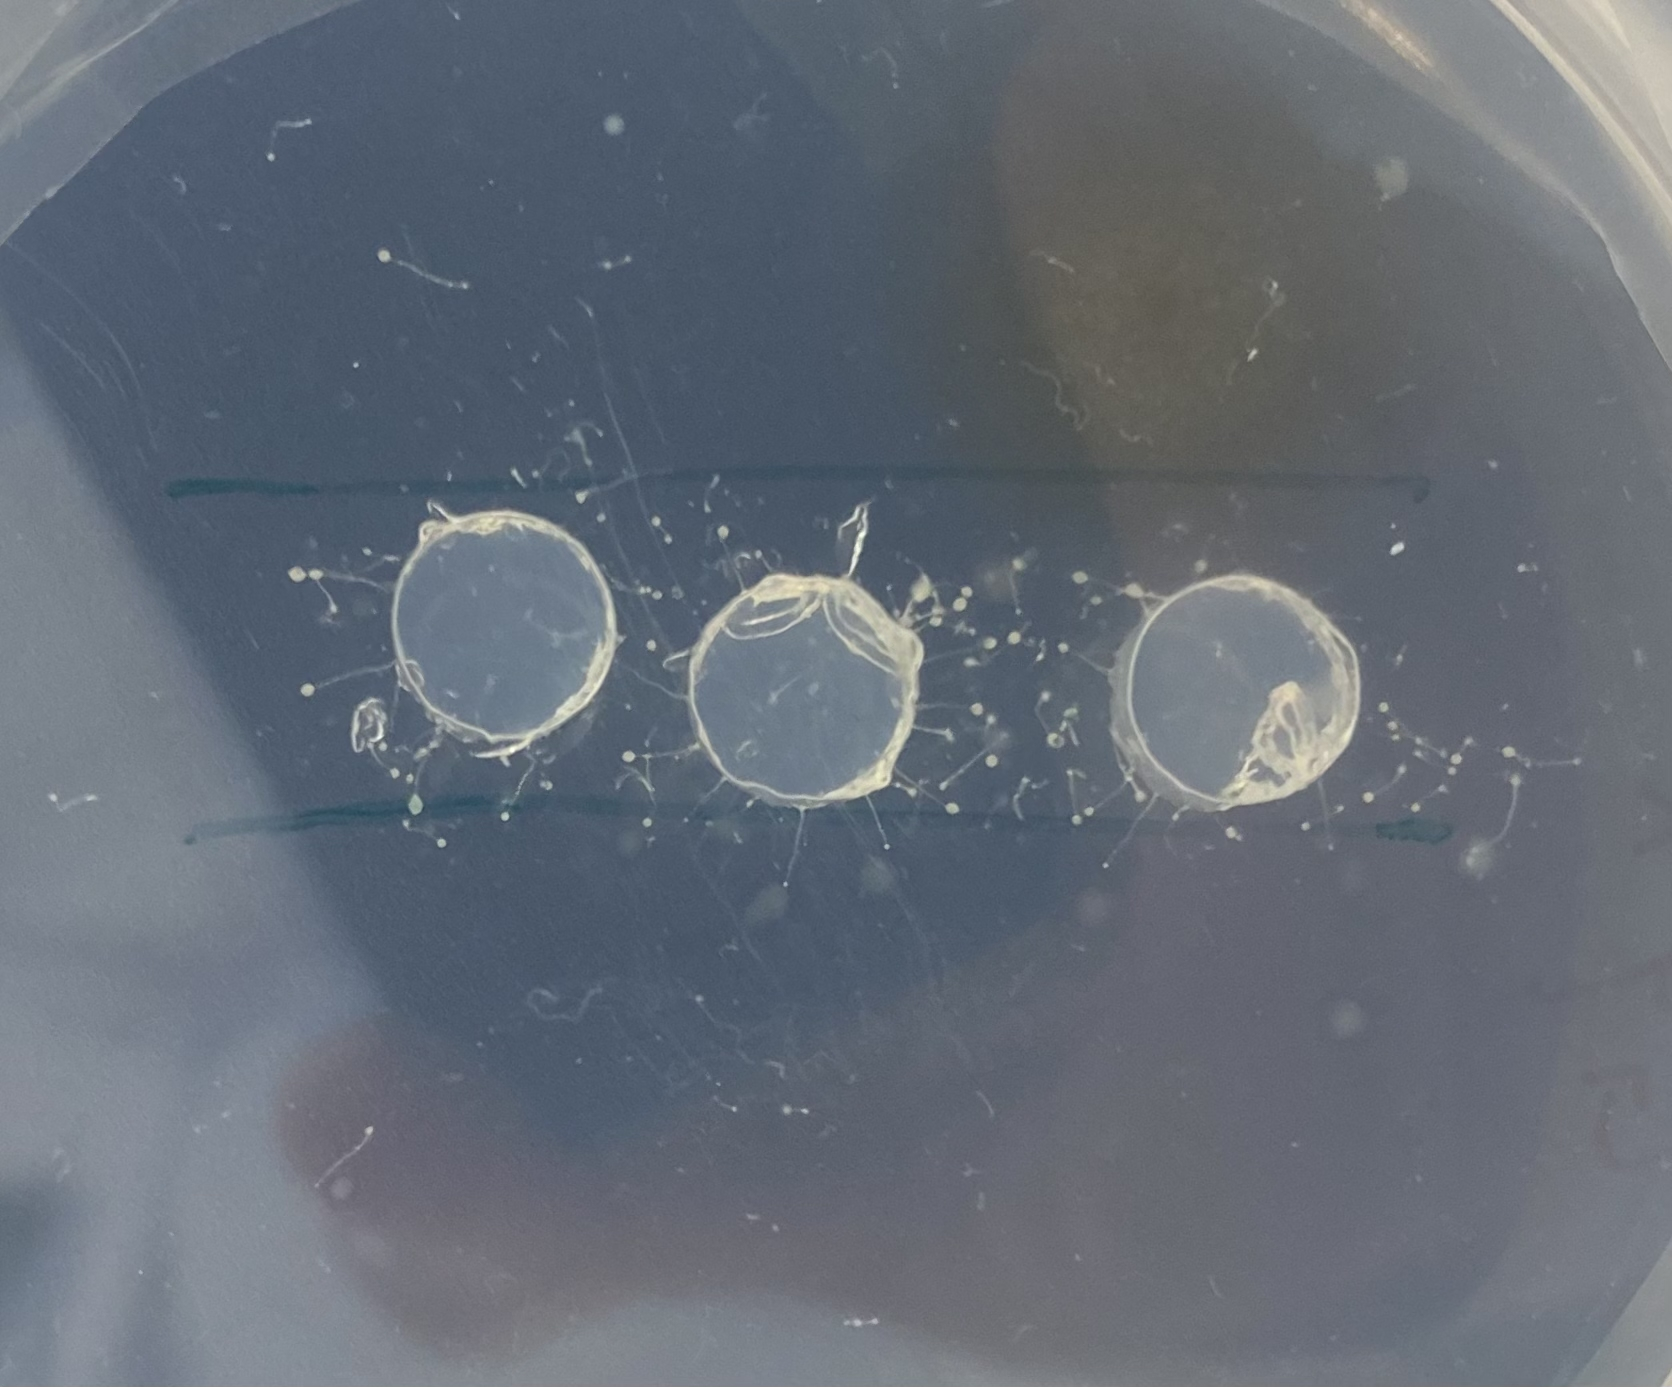
\includegraphics[width=0.26\textwidth, height=0.25\textwidth]{figures/p1.jpg}}
    \caption{Fruiting in \textsl{Dictyostelium}. (a) Non-nutrition agar with \textsl{E.coli}. The white band is the \textsl{E.coli} bacteria smeared on the NNA. (b) Non-nutrition agar with \textsl{E.coli} and \textsl{Dictyostelium}. The three discs were cut from the \textsl{Dictyostelium} stock and inverted into the \textsl{E.coli} band.}
    \label{fig:my_label}
\end{figure}
